\section{Applications of EVT Analysis}
Representing the angular component of the Pareto process with a (semi) parametric distribution grants
  us opportunities in posterior analysis.

\subsection{Face Probabilities}
One of the simplest inferences we can make from this model would be the probability of a particular
  dimension being max--the probability of falling on a particular face.  This provides us an
  understanding on which dimensions are more likely to be extreme.
  \begin{equation}
    \text{P}\left(Z_l = \max_{i}Z_i\right) = \text{P}\left(V_l = 1\right) = \text{E}\left[1_{V_l = 1}\right]
  \end{equation}
  Even in the gamma case, this is difficult to calculate directly. Were we to find an analytic form
  of this quantity, we could approach the problem of establishing a density on $\mathcal{S}_{\infty}^{d-1}$
  in the manner outlined in Eqn.~\ref{eqn:mixconddensity}.  However, we can calculate this via
  Monte Carlo integration; in much the same manner as we will calculate the other inferences in this
  section.

\subsection{Pairwise Extremal Dependence Coefficients}
A summary measure of extremal dependence between dimensions can be offered by the extremal dependence
  coefficient.  This can be thought of as something like a correlation coefficient for extreme
  observations.  For a random variable $\bm{Z}$, which has been standardized such that the marginal
  distributions are common between dimensions, it is defined as
  \begin{equation}
    \chi_{kl} = \lim\limits_{u\to\infty}\text{P}\left(Z_k > u\mid Z_l > u\right).
  \end{equation}
  The value $\chi_{kl} \in [0,1]$.  When $\chi_{kl}$ approaches 1, that indicates complete dependence;
  the variables are linked, in much the same manner as if a correlation coefficient approaches 1.
  When $\chi_{kl}$ is greater than 0, $X_k$ and $X_l$ are considered asymptotically dependent.  For
  a $\bm{Z}$ distributed by a Pareto process, Warner and Sans{\'o}\cite{warner2018} transform $Z$
  to the unit square to re-express this quantity,
  \begin{equation}
    \label{eqn:extdepcoef}
    \chi_{kl} = \text{E}\left[\frac{V_k}{\text{E}(V_k)}\wedge\frac{V_l}{\text{E}(V_l)}\right]
  \end{equation}
  for $V_k,V_l \in [0,1]$.  This calculation is wholely dependent on the angular component, as radial
  measure is independent of angular measure.  Important to note, however, is that complete asymptotic
  independence, where $\chi_{kl} := 0$, can not be described under a Pareto process based model.

  \begin{figure}[h]
    \centering
    \label{fig:chi_ij}
    \begin{minipage}{.5\textwidth}
      \centering
      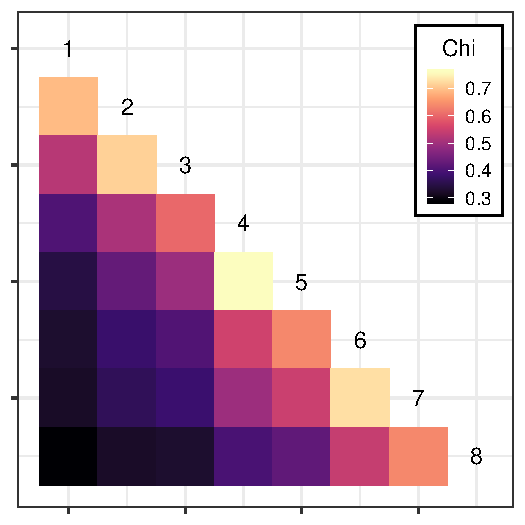
\includegraphics{./images/chi_ij_8}}
    \end{minipage}
    \begin{minipage}{.5\textwidth}
      \centering
      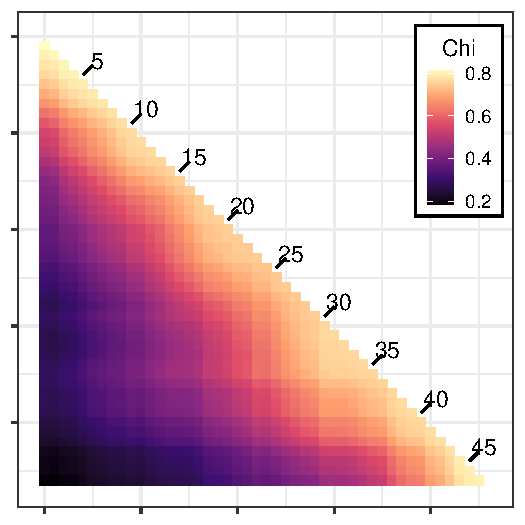
\includegraphics{./images/chi_ij_46}
    \end{minipage}
    \caption{Pairwise extremal dependence coefficients for IVT data, computed from fitted DP mixture
      of projected restricted gamma model.  The left corresponds to the 8-cell data, the right the
      46-cell data.}
  \end{figure}

Figure~\ref{fig:chi_ij} plots the pairwise extremal dependence coefficients for the IVT data, in 8
  cells (left) and 46 cells (right), computed fom a fitted DP mixture of projected restricted gammas.
  We see a higher extremal dependence between neighboring columns which is not unexpected, as
  neighboring columns correspond to neighboring cells.  We recognize that pairwise asymptotic dependence
  coefficients tell a limited story, as a particular dependence may structure may include more than
  two columns.   We can, however, glean some information from the patterns that emerge in two dimensions.
  On the 8-cell data, we see a stronger association between columns 5,6,7, indicating a greater
  dependence among these columns.  On the 47 cell data, we see at least 3 groupings of columns,
  indicating greater asymptotic dependence among these groups.

\subsection{Conditional Survival Curves}
Another interesting inference we can make from a fitted model is a conditional survival curve.
  Following rules of conditional probability, we can develop survival curves based on
  threshold exceedences. For ${\bf Z} = (Z_1,\ldots,Z_d)$ following a $d$-variate Pareto distribution,
  In 1 dimension, the conditional survival function can be developed as
  \begin{equation}
    \label{eqn:condsurv1d}
    \text{P}\left(Z_l > z_l\mid {\bf Z}_{-(l)} > {\bf z}_{-(l)}\right) =
      \frac{\text{P}\left(\cap_{k = 1}^d Z_k > z_k\right)}{\text{P}\left(\cap_{k \neq l} Z_k > z_k\right)}.
  \end{equation}
  Let $R = \pnorm{{\bf Z}}{\infty}$, ${\bf V} = \frac{{\bf Z}}{R}$, such that ${\bf V}\in \mathcal{S}_{\infty}^{d-1}$.
  For evaluating these probabilities, recall that ${\bf Z} = R{\bf V}$.  Then,
  \begin{equation}
    \text{P}\left(\cap_{k = 1}^d Z_k > z_k\right) = \text{P}\left(\cap_{k = 1}^d RV_k > z_k\right)
  \end{equation}
  Also, for standard Pareto, recall that $\text{P}(R > r) = 1\wedge\frac{1}{r}$.  Then,
  \begin{equation}
    \text{P}\left(\cap_{k = 1}^d R > \frac{z_k}{v_k}\right) =
      \text{P}\left(R  > \vee_{k=1}^d\frac{z_k}{V_k}\right) =
      \text{E}\left[1 \wedge \left(\vee_{k = 1}^d\frac{z_k}{V_k}\right)^{-1}\right].
  \end{equation}
  As $V_k \in [0,1]$, and given our interest in the tail of the distribution, we can assume $z_k > 1$,
  therefore $\frac{z_k}{V_k} > 1$.  We thus arrive at
  \begin{equation}
    \text{P}\left(\cap_{k = 1}^dZ_k > z_k\right) = \text{E}\left(\wedge_{k = 1}^d\frac{V_i}{z_i}\right).
  \end{equation}
  We employ a similar calculation in the denominator, and arrive at
  \begin{equation}
    \label{eqn:condsurv1df}
    \text{P}\left(Z_l > z_l\mid {\bf Z}_{\neg(l)} > {\bf z}_{\neg(l)}\right) =
      \frac{\text{E}\left[\wedge_{k = 1}^d \frac{V_k}{z_k}\right]}{\text{E}\left[\wedge_{k \neq l}\frac{V_k}{z_k}\right]}.
  \end{equation}
  Following similar calculations, for a dimension set $\alpha \subset \{1,\ldots, d\}$, a multivariate
  conditional survival function can be similarly estimated as
  \begin{equation}
    \label{eqn:condsurv2df}
    \text{P}\left(\cap_{l \in \alpha} Z_l > z_l \mid \cap_{l\not\in\alpha} Z_l > z_l\right) =
      \frac{\text{E}\left[\wedge_{k = 1}^d \frac{V_k}{z_k}\right]}{\text{E}\left[\wedge_{k \not\in\alpha}\frac{V_k}{z_k}\right]}.
  \end{equation}
  We will be presenting single- and bi-variate forms of these curves.   Given appropriate values of
  ${\bf z}$, we can generate these curves from samples from the posterior predictive distribution of
  a fitted model.

\begin{figure}[h]
  \label{fig:condsurv1d}
  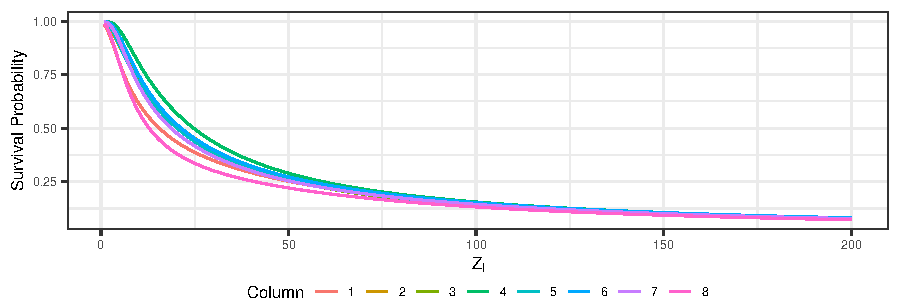
\includegraphics{./images/condsurv_1d}
\end{figure}

\begin{figure}[h]
  \label{fig:condsurv_2d}
  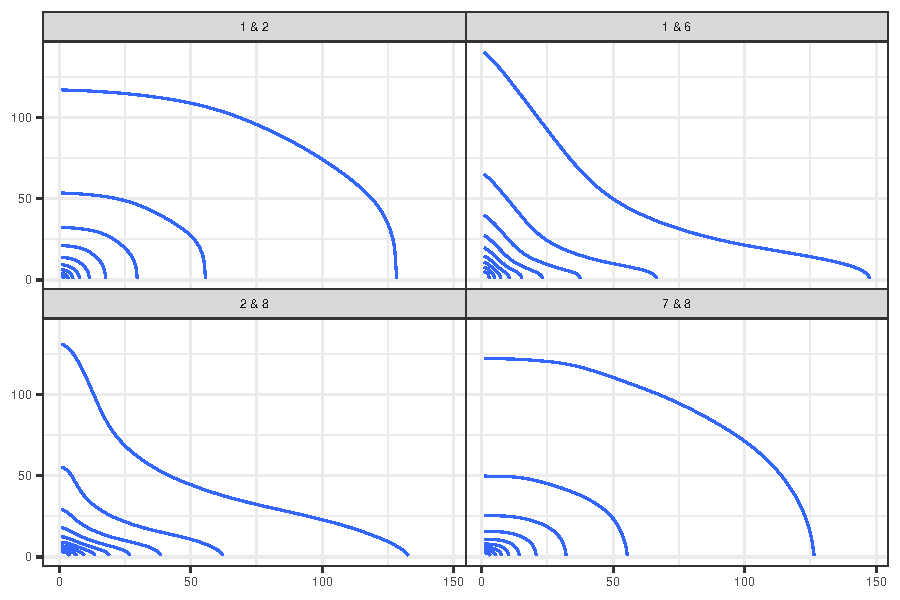
\includegraphics{./images/condsurv_2d}
\end{figure}









% EOF
